\documentclass[11pt]{article}
\usepackage[utf8]{inputenc}
\usepackage{geometry}
 \geometry{
 a4paper,
 left=25mm,
 top=20mm,
 bottom=20mm,
 right=15mm
 }
 \usepackage{amsmath}
 \usepackage{pgfplots} % per a graficar amb LaTeX
\pgfplotsset{samples=2000} % número màxim de punts d'una corba que genera ell, canviar
\pgfplotsset{compat=1.16} % perquè si no el pgfplot dóna error
\usepackage{import} % per a les imatges d'Inkscape
\usepackage{xifthen} % per a les imatges d'Inkscape
\usepackage{pdfpages} % per a les imatges d'Inkscape
\usepackage{transparent} % per a les imatges d'Inkscape
\usepackage[RPvoltages]{circuitikz} % per tal que no salti warning
\usetikzlibrary{arrows, decorations.markings, arrows.meta} % per a dibuixar fletxes d'intensitat
\usepackage{gensymb}
\usepackage{steinmetz}


\begin{document}

Given a simple system like the one in Figure \ref{fig:sistema} I wish to solve the power flow using the Flexible General Branch Model.
\begin{figure}[!htb]
    \begin{center}
    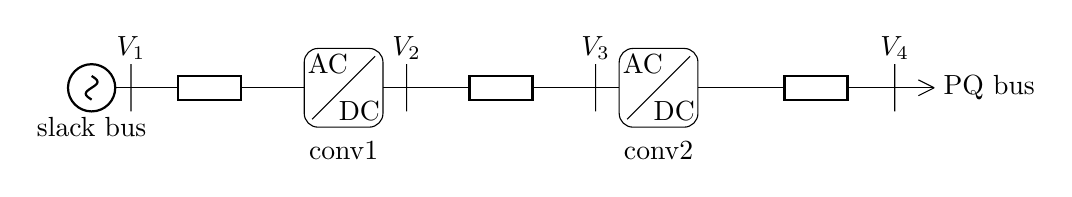
\begin{tikzpicture}[scale = 1, transform shape]
        \draw (-2, 0) to [/tikz/circuitikz/bipoles/length=1.0cm, sV] (-1.4, 0);
        \ctikzset{resistor = european}
        \draw (-1.4, 0) to [/tikz/circuitikz/bipoles/length=1.0cm, resistor] (1, 0);
        \draw[rounded corners=5pt] (1,-0.5) rectangle (2.0,0.5);
        \draw (1.1,-0.4) -- (1.9,0.4);
        \node at (1.3,0.3) {AC};
        \node at (1.7,-0.3) {DC};
        \draw (2, 0) to [/tikz/circuitikz/bipoles/length=1.0cm, resistor] (5, 0);
        \draw[rounded corners=5pt] (5,-0.5) rectangle (6.0,0.5);
        \draw (5.1,-0.4) -- (5.9,0.4);
        \node at (5.3,0.3) {AC};
        \node at (5.7,-0.3) {DC};
        \draw (6, 0) to [/tikz/circuitikz/bipoles/length=1.0cm, resistor] (9, 0);
        \draw (9, 0) to [short] (8.8, 0.1);
        \draw (9, 0) to [short] (8.8, -0.1);
        \draw (-1.2, 0.3) to [short] (-1.2, -0.3);
        \draw (2.3, 0.3) to [short] (2.3, -0.3);
        \draw (4.7, 0.3) to [short] (4.7, -0.3);
        \draw (8.5, 0.3) to [short] (8.5, -0.3);
        \node at (-1.2, 0.5) {$V_1$};
        \node at (2.3, 0.5) {$V_2$};
        \node at (4.7, 0.5) {$V_3$};
        \node at (8.5, 0.5) {$V_4$};
        \node at (5.5, -0.8) {conv2};
        \node at (1.5, -0.8) {conv1};
        \node at (9.7, 0.0) {PQ bus};
        \node at (-1.7, -0.5) {slack bus};
    \end{tikzpicture}
    \caption{Simplified system with the AC/DC converter}
    \label{fig:sistema}
    \end{center}
    \end{figure}

Now, the consideration is that converter 1 (conv1) operates following control mode 5 whereas converter 2 (conv2) uses the control mode 2. Thus, $|V_2|$ and the active power leaving bus 3 that goes through conv2 (we will call it $P_f$) correspond to data I specify. 

As I understand it, I encounter the next unknowns: $\delta_2$, $\delta_3$, $\delta_4$, $|V_3|$, $|V_4|$, $m_{a,1}$, $B_{eq,2}$ and $\theta_{sh,2}$. My guess is that the control variable $m_a$ has to be found only for conv1 because we control $|V_2|$ while $B_{eq}$ and $\theta_{sh}$ are related to conv2 in this case due to the fact that it operates in control mode 2.

I then take into consideration equations \ref{eq:1} and \ref{eq:2} for buses 2, 3 and 4:
\begin{equation}
    \sum P = 0,
    \label{eq:1}
\end{equation}
\begin{equation}
    \sum Q = 0.
    \label{eq:2}
\end{equation}
So there are two equations left to construct a system of 8 equations and 8 unknowns. Let's say $i_{34}$ is the current leaving bus 3 in direction to bus 4. As a result of that we have:
\begin{equation}
    V_3i^*_{34} = P_f + j0.
\end{equation}
To my surprise, the jacobian involved in solving the nonlinear system of equations becomes singular. 

\end{document}